\documentclass[11pt,a4paper]{article}
\usepackage{lmodern}
\usepackage[T1]{fontenc}
\usepackage{amsmath,amssymb}
\usepackage{graphicx}
\usepackage{longtable,booktabs,array}
\usepackage{float}
\usepackage[margin=25mm]{geometry}
\usepackage{caption}
\usepackage{hyperref}
\hypersetup{colorlinks=true,linkcolor=blue,urlcolor=blue,citecolor=blue}
\setkeys{Gin}{width=0.82\linewidth,keepaspectratio}
\usepackage{amsthm}
\newtheorem{theorem}{Theorem}
\newtheorem{proposition}{Proposition}
\newtheorem{lemma}{Lemma}
\newtheorem{corollary}{Corollary}
\newtheorem{definition}{Definition}
\newtheorem{remark}{Remark}
\newtheorem{observation}{Observation}
\usepackage{calc}
\newcounter{none}
\providecommand{\real}[1]{#1}
\providecommand{\pandocbounded}[1]{#1}
\providecommand{\tightlist}{\setlength{\itemsep}{0pt}\setlength{\parskip}{0pt}}
\title{Simulated Observation of the de Broglie Wavelength in a Localized
Odd-Harmonic Double-Slit Model}
\author{Noriaki Kihara, WF System Co., Ltd.~--- DOI:
10.5281/zenodo.21109903}
\date{v0.3 --- July 2026}
\begin{document}
\maketitle
\emph{------ Interference-survival condition of a highly localized
structure, and the fundamental-wavelength invariance of the observed
wavelength}

\section{Abstract}\label{abstract}

The de Broglie wavelength \(\lambda=h/p\) was first confirmed by the
1927 Davisson--Germer electron diffraction {[}2{]}. This paper is a
numerical experiment that \textbf{simulates and observes} this relation
inside a \textbf{single-source double-slit classical wave model} (the
interference and alignment judgement are deterministic; only the input
position and wavelength fluctuations are supplied by independent Monte
Carlo draws). The electron is modeled as a \textbf{spatially localized
wave} with representative wavelength \(\lambda_0=h/p\), composed of an
equal-amplitude sum of odd harmonics for \(N>1\) {[}1{]} (as noted
below, this is not the electron wave packet itself but a classical
analogue: the minimal Fourier construction of a spatially localized
pulse). Computing the exact two-slit interference at the physical scale
(\(L=5\,\mathrm{cm}\), \(W=5\,\mu\mathrm{m}\)): for \(N=1\) the wave
always interferes and the fringe spacing recovers \(\lambda_0\) (a check
of the procedure). For \(N>1\), preserving the localized shape requires
an inter-harmonic alignment condition (the geometric resonance
\(r_{\mathrm{avg}}/\lambda=M/2\)); at wavelengths that do not satisfy
it, the localization collapses and no stable fringes form. Computing
each electron exactly under a symmetric fluctuation centered at
\(\lambda_0=h/p\), the effective wavelength \(\lambda'\) that interferes
stably is selected as the nearest resonance. \textbf{The central result
of this paper is not the value of \(h\).} The resonance-lattice spacing
is \(\sim10^{-19}\,\mathrm{m}\)---so dense that
\(\lambda'\approx\lambda_0\) (relative \(\sim10^{-9}\)), and
\(p\lambda'\approx h\) is a nearly tautological self-consistency. The
center of gravity of this paper is the \textbf{interference survival of
the structure and the fundamental-wavelength invariance of the observed
wavelength}: even when finer localized structure (\(N>1\) odd harmonics)
than \(\lambda_0\) is packed in, the wave can \textbf{``survive''}
two-slit interference as a sharp single peak, and the observed central
fringe spacing remains at the fundamental wavelength \(\lambda_0\)
(\(N\) controls only the sharpness of localization \(\sim1/(N{+}1)\)).
This fundamental-wavelength invariance is a \textbf{structural} result,
independent of whatever physical origin the fundamental wavelength
\(\lambda_0\) is given; it is a claim distinct from the numerical
recovery of \(h\). \textbf{This paper is neither a first-principles
derivation of \(p\lambda=h\) nor a derivation of a
\(\Delta x\,\Delta p\sim h\) type uncertainty relation.} As a guard
against misreading, each electron is given an independent Monte Carlo
draw of its source position (\(\cos^2\), \(\pm\lambda_0/2\)) and its
initial wavelength (\(\cos^2\), \(\pm1\%\)), and the interference,
alignment, and exclusion are recomputed exactly at each
\((y,\lambda_0')\). Under this symmetric fluctuation centered at
\(\lambda_0=h/p\), \(\langle p\lambda'\rangle\) agrees with \(h\) within
the standard error (sample standard deviation \(\sigma\approx0.36\%\) =
the theoretical value of the \(\cos^2\) distribution, SE
\(\approx\sigma/\sqrt{n_{\mathrm{OK}}}\)); a few percent of trials whose
\(\lambda_0'\) falls near a resonance midpoint are excluded by the
extraction procedure.

\begin{center}\rule{0.5\linewidth}{0.5pt}\end{center}

\section{1. Introduction and scope}\label{introduction-and-scope}

In 1924--1925 de Broglie associated a wavelength \(\lambda=h/p\) with a
particle {[}3{]}. This relation was confirmed by the Davisson--Germer
nickel electron diffraction {[}2{]} (Bragg condition
\(n\lambda=2d\sin\theta\): with known \(d\) and measured \(\theta\),
\(\lambda\) is obtained and compared with \(h/p\)).

Scope of this paper:

\begin{itemize}
\tightlist
\item
  \textbf{Not} a proposal of a new measurement method, nor a
  re-measurement of a real experiment.
\item
  \textbf{Not} a first-principles derivation of \(p\lambda=h\) (§5.1,
  §5.2).
\item
  It is a \textbf{numerical experiment in classical wave optics}
  borrowing the two-slit geometry, asking: what alignment condition does
  a \textbf{highly localized} classical wave (\(N>1\) odd harmonics)
  with a de Broglie-scale representative wavelength require to survive
  stably as sharp interference under two-slit geometry, and how is the
  observed wavelength scale preserved.
\end{itemize}

Davisson--Germer used a crystal ``lattice'', whereas this model uses a
double slit. But whereas the real experiment supplies \(\lambda\)
independently via the \textbf{external measured datum} of the
diffraction angle, this model generates fringes from \(\lambda_0=h/p\)
and reads them back, so it does not have an independent measurement path
and is not isomorphic in that sense (§5.3). The novelty of this paper
is: applying the localized odd-harmonic / alignment condition of {[}1{]}
to \textbf{the double-slit geometry}, performing \textbf{per-electron
exact alignment/exclusion judgement} under \textbf{independent Monte
Carlo} of position and wavelength, and statistically verifying the
\textbf{fundamental-wavelength invariance} of the observed wavelength.

\begin{center}\rule{0.5\linewidth}{0.5pt}\end{center}

\section{2. Model definition and
computation}\label{model-definition-and-computation}

\subsection{2.1 Geometry}\label{geometry}

Source--slit distance \(L=5\,\mathrm{cm}\), slit separation
\(W=5\,\mu\mathrm{m}\), slits at \(y_{\mathrm{slit}}=\pm W/2\). For a
source position \(y\) (which fluctuates, below) the two path lengths are
\[r_1(y)=\sqrt{L^2+(y-W/2)^2},\quad r_2(y)=\sqrt{L^2+(y+W/2)^2},\quad r_{\mathrm{avg}}=\tfrac{r_1+r_2}{2}.\]
At the centred source \(y=0\),
\(r_1=r_2=r_{\mathrm{avg}}=\sqrt{L^2+(W/2)^2}\). At the physical scale
the characteristic lengths differ by orders of magnitude
(\(W/\lambda_0\sim5\times10^4\), \(L/W\sim10^4\),
\(L/\lambda_0\sim5\times10^8\)), making a common-scale drawing
impossible, and the half-angle
\(\theta=\arctan[(W/2)/L]\approx2.9\times10^{-3}{}^\circ\) is extremely
paraxial.

\pandocbounded{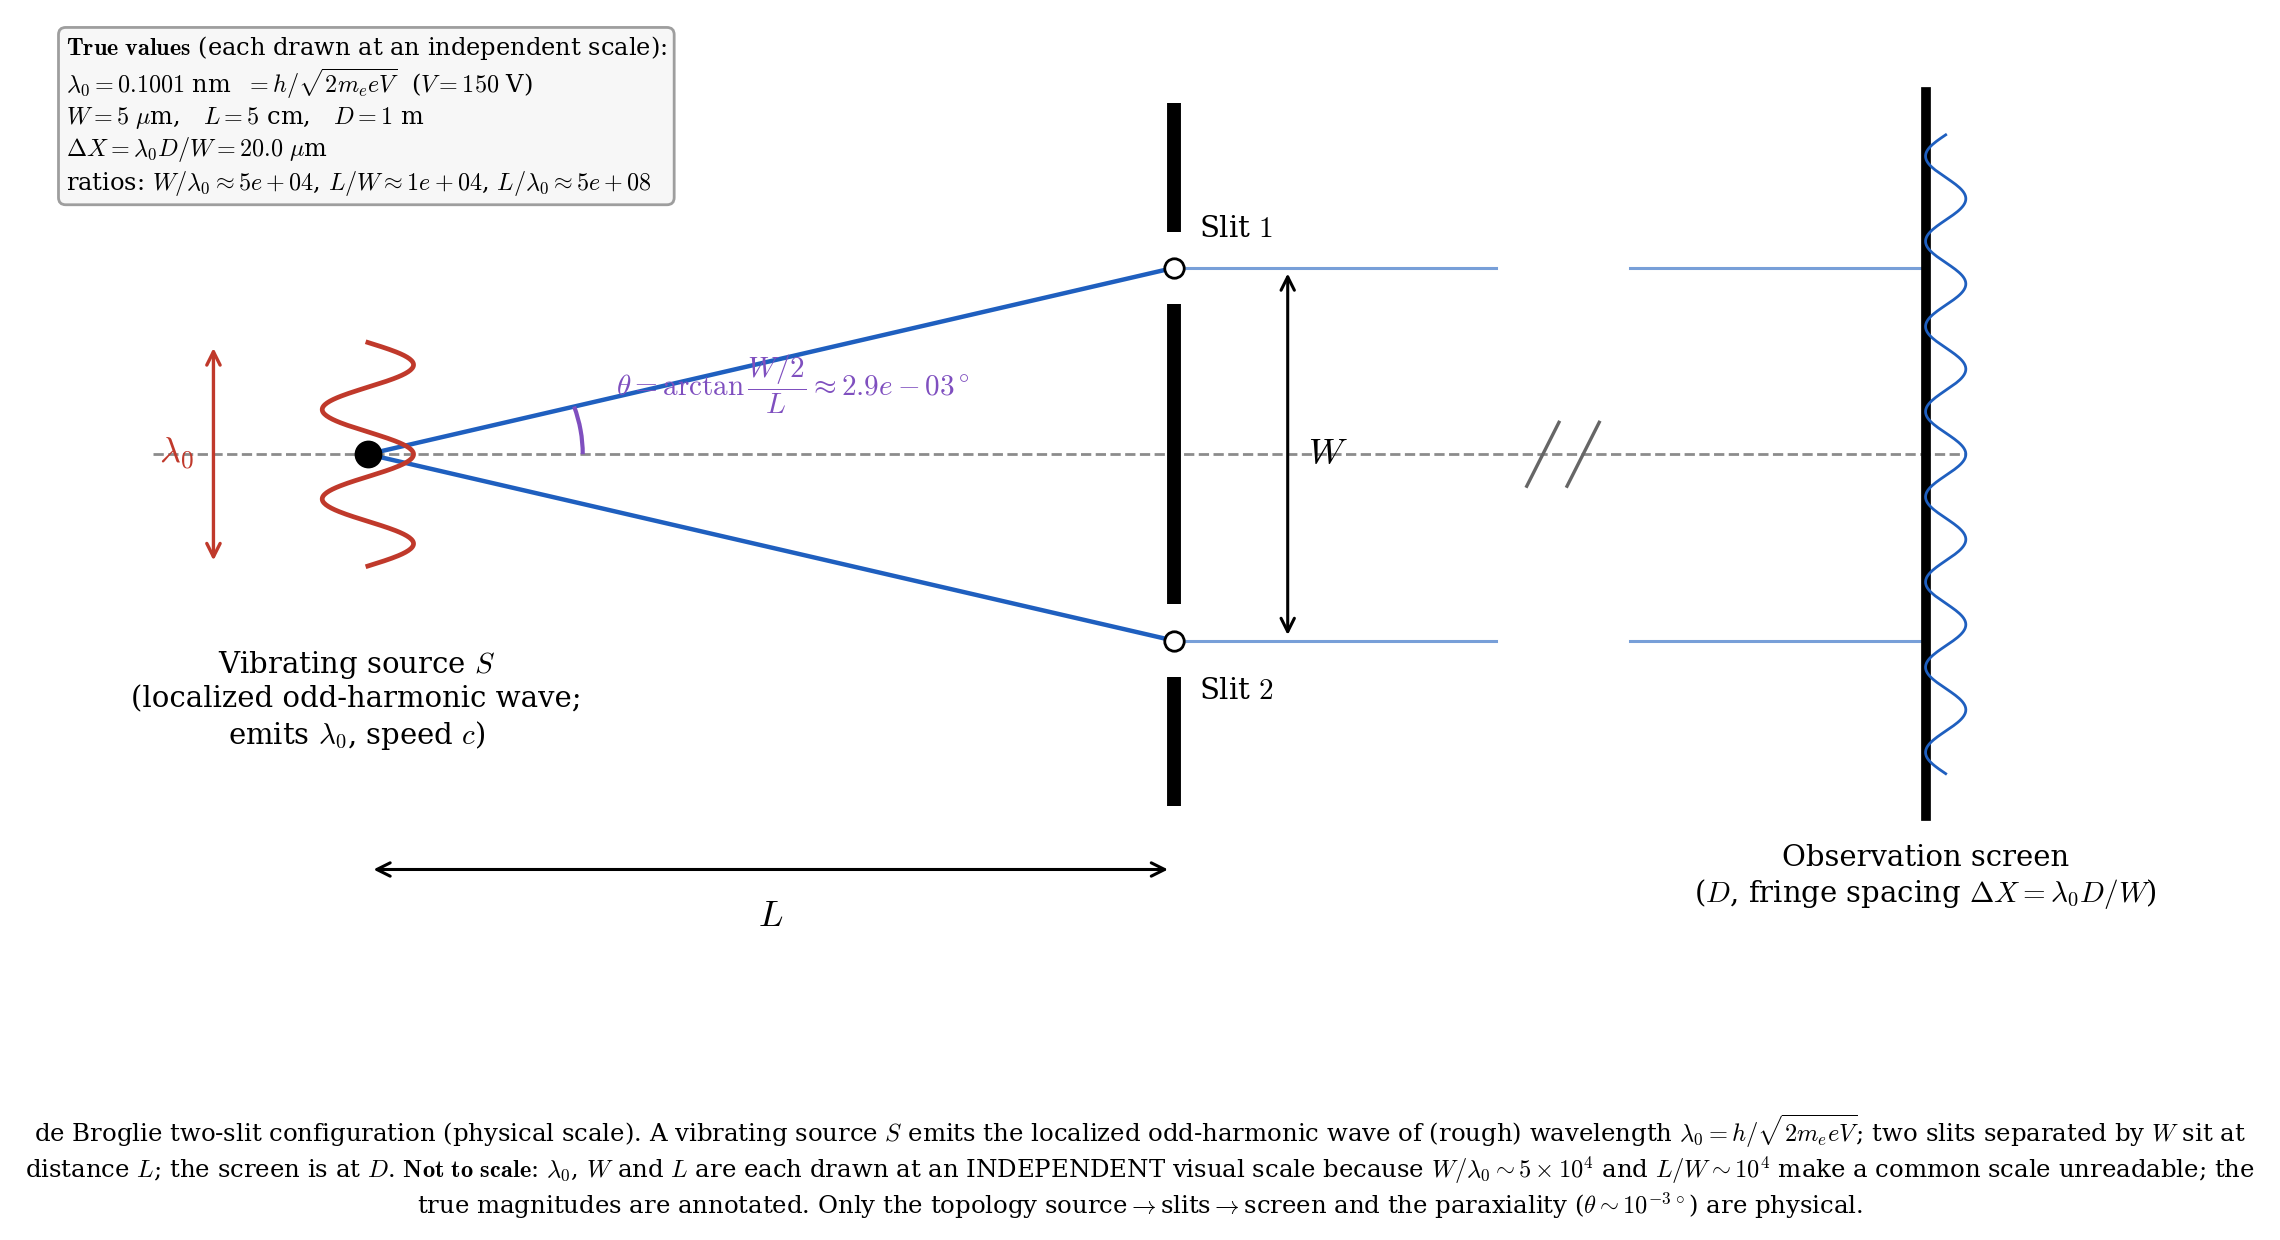
\includegraphics[keepaspectratio,alt={Figure 1}]{fig_setup_debroglie_V150.png}}
\textbf{Figure 1}: Schematic of the setup (\(V=150\,\mathrm{V}\)).
\(\lambda_0,W,L\) are each drawn at an independent scale (the top-left
box notes the true ratios \(W/\lambda_0\approx5\times10^4\), etc.). Only
the topology and the paraxiality \(\theta\sim10^{-3\,\circ}\) are
physical; the size ratios are exaggerated (§2.1).

\subsection{2.2 The localized odd-harmonic wave and the exact
intensity}\label{the-localized-odd-harmonic-wave-and-the-exact-intensity}

\textbf{Physical motivation}: for convenience we call it the
``electron'' below, but what we compute is not the full quantum state of
an electron; it is a trial of a classical localized wave whose
representative wavelength is at the de Broglie scale. This model treats
that localized wave as a \textbf{spatially localized pulse wave}, not a
point without spatial extent. An equal-amplitude sum of odd harmonics is
the minimal Fourier construction that gives a symmetric localized peak
at the center \(s=0\) {[}1{]}, and excluding the even components
preserves the symmetry. \textbf{Note}: these odd-harmonic components do
\textbf{not} mean the different momentum eigenstates of a free electron
in standard quantum mechanics (a factor-\(n\) wavenumber would mean
momentum \(np\) and energy \(n^2E\)); they are \textbf{Fourier
components in a classical wave model used to construct the localized
shape}. Moreover, this paper is not a time-evolving quantum wave-packet
model but a \textbf{stationary classical wave model that inspects the
spatial phase structure on the screen}; the energy dispersion of the
harmonic components and temporal decoherence are out of scope.

Wavenumber components \(n=1,3,\dots,N\) (\(\lambda_n=\lambda/n\),
\(K=(N{+}1)/2\) of them). The exact screen intensity after the two slits
is
\[I(s;y)=\Big|\sum_{n=1,3,\dots,N}\big(e^{i\Phi_1^{(n)}}+e^{i\Phi_2^{(n)}}\big)\Big|^2,\qquad
\Phi_k^{(n)}=\frac{2\pi n}{\lambda}\big(r_k-y_{\mathrm{slit},k}\,s\big),\]
where \(s\) is the paraxial screen variable (\(s\simeq X/D\) for the
far-field coordinate \(X\)). Numerically we use the algebraically
equivalent factored form
\[e^{i\Phi_1^{(n)}}+e^{i\Phi_2^{(n)}}=e^{i\,2\pi n\,r_{\mathrm{avg}}/\lambda}\cdot2\cos\!\Big(\pi n\frac{(r_1-r_2)-Ws}{\lambda}\Big),\quad r_1-r_2=\frac{-2Wy}{r_1+r_2}\]
(the physics is unchanged; this avoids cancellation at absolute phases
\(\sim10^9\,\mathrm{rad}\)). \textbf{In this form,
\(e^{i2\pi n r_{\mathrm{avg}}/\lambda}\) carries the inter-harmonic
absolute alignment, while \(\cos(\pi n[(r_1-r_2)-Ws]/\lambda)\) carries
the relative phase of the two-path interference.} That is, the dominant
factor observed in an ordinary double slit is the path difference
(relative phase), but in this model an \textbf{additional harmonic
alignment with respect to the absolute mean distance
\(r_{\mathrm{avg}}\)} is required to preserve the localized odd-harmonic
shape at the center.

\subsection{\texorpdfstring{2.3 The central alignment \(A(\lambda)\)
(absolute
measure)}{2.3 The central alignment A(\textbackslash lambda) (absolute measure)}}\label{the-central-alignment-alambda-absolute-measure}

The intensity at the screen center \(s=0\) is
\(I(0)=\big|2\sum_n e^{i2\pi n r_{\mathrm{avg}}/\lambda}\big|^2=4K^2A(\lambda)\),
\[A(\lambda)=\frac{1}{K^2}\Big|\sum_{n=1,3,\dots,N}e^{i2\pi n\,r_{\mathrm{avg}}/\lambda}\Big|^2.\]
\(A\) is the \textbf{fraction of full alignment}: \(A=1\)
(\(I(0)=4K^2\)) only at a true resonance
(\(r_{\mathrm{avg}}/\lambda=M/2\)) where all odd-harmonic phases align,
and \(A<1\) otherwise. As noted, \(A\) is the measure of the above
(absolute) alignment, i.e.~it measures \textbf{the preservation
condition of the localized shape}. Because \(A\) is referred to the
absolute maximum \(4K^2\) fixed by geometry and \(N\), a degraded
partially-aligned pattern gives \(A\ll1\) and is correctly rejected (a
self-normalized \(I(0)/I_{\max}\) cannot make this distinction).

\subsection{2.4 Independent per-electron fluctuations and exact
computation}\label{independent-per-electron-fluctuations-and-exact-computation}

To emulate real apparatus fluctuations, \textbf{each electron (trial) is
given two independent Monte Carlo draws}:

\begin{enumerate}
\def\labelenumi{\arabic{enumi}.}
\tightlist
\item
  \textbf{Source position} \(y\sim\cos^2(\pi y/\Delta)\), range
  \(\pm\Delta/2\) (\(\Delta=\lambda_0\), peaked at the center \(0\)).
\item
  \textbf{Initial wavelength} \(\lambda_0'=\lambda_0+\eta\),
  \(\eta\sim\cos^2(\pi\eta/2\delta)\), \(\delta=0.01\,\lambda_0\)
  (\(\pm1\%\), drawn from a random stream independent of position).
\end{enumerate}

The two draws are independent, hence statistically uncorrelated (no
spurious correlation between position and wavelength). For each
electron, using the geometry \(r_{\mathrm{avg}}(y)\) of its
\((y,\lambda_0')\), the interference, alignment, and exclusion are
computed \textbf{exactly every time} (no \(y=0\)-fixed or
\(\lambda_0\)-fixed approximation; for \(N=9\) this is about
\(4\times10^4\) evaluations of \(A\) per voltage point). The theoretical
standard deviation of the \(\cos^2\) distribution is
\(\sigma=\delta\sqrt{1/3-2/\pi^2}\approx0.362\,\delta\),
i.e.~\textbf{\(\sigma\approx0.362\%\)} for a \(\pm1\%\) input.

\subsection{\texorpdfstring{2.5 Search for the effective wavelength
\(\lambda'\) and the exclusion
judgement}{2.5 Search for the effective wavelength \textbackslash lambda\textquotesingle{} and the exclusion judgement}}\label{search-for-the-effective-wavelength-lambda-and-the-exclusion-judgement}

For each electron, within the \textbf{geometric window}
\([\lambda_0'-\lambda_0'^2/(4r_{\mathrm{avg}}),\ \lambda_0'+\lambda_0'^2/(4r_{\mathrm{avg}})]\)
(= half the resonance spacing) around \(\lambda_0'\), sweep
\(A(\lambda)\) and count the connected bands with \(A\ge0.98\)
(resonance bands). If there is exactly one band, refine its peak by
golden-section search to obtain the effective wavelength
\(\lambda'=2r_{\mathrm{avg}}/M\) (satisfying \(A(\lambda')=1\),
\(I(0)=4K^2\) to machine precision). If there are zero or two-or-more
bands (near a resonance midpoint, the nearest resonance is not unique
for \(\lambda_0'\)), that trial is excluded. The window width and the
alignment condition are determined by geometry alone; \(h\) enters only
through the center \(\lambda_0=h/p\) of \(\lambda_0'\). The observed
order \(M=\mathrm{round}(2r_{\mathrm{avg}}/\lambda')\) is a post-hoc
output (the symbol \(M\) for the order is distinguished from the
electron mass \(m_e\)).

\textbf{Physical interpretation of the ``alignment (snap)''
(important)}: the alignment in this model does \textbf{not} claim a
mechanism by which the source physically changes its wavelength after
emission (e.g.~injection locking via backscatter from the slits). It is
an operation that \textbf{mathematically stands in for the survival bias
(filtering) that ``only wavelengths that align form a stable single-peak
fringe, while the rest form no fringe''}. The exclusion (the ``band
\(\neq1\)'' trials of the previous paragraph) is a part of this filter
(removal of trials for which the nearest resonance cannot be uniquely
chosen); it is a \textbf{procedural judgement dependent on the threshold
0.98 and the window width}, and does not mean the electron physically
disappears (the rate is set by the threshold, not by nature). By
``survival'' in this paper we mean that a stable single-peak fringe is
extractable, not the physical life or death of an electron.

\subsection{\texorpdfstring{2.6 The role of \(\lambda_0\) and the
positions of \(N=1\) /
\(N>1\)}{2.6 The role of \textbackslash lambda\_0 and the positions of N=1 / N\textgreater1}}\label{the-role-of-lambda_0-and-the-positions-of-n1-n1}

\(\lambda_0=h/p\) is the initial condition of the interference
computation; without \(\lambda_0\) the phase \(2\pi r/\lambda\) cannot
be defined. Since \(\lambda_0\) itself is given using \(h\), the
recovery of \(p\lambda'\) is not an independent derivation of \(h\) but
a self-consistency check.

\begin{itemize}
\tightlist
\item
  \textbf{\(N=1\) (single harmonic)} always interferes without an
  alignment condition, and the same \(\lambda_0\) is recovered from the
  fringe spacing. Hence \(N=1\) is not a physical discovery but a
  \textbf{check of the computation and the wavelength-readout
  procedure}.
\item
  \textbf{\(N>1\) (localized odd-harmonic wave)} is the main subject.
  This waveform has structure finer than \(\lambda_0\), and it can
  interfere stably only on the discrete resonances
  \(r_{\mathrm{avg}}/\lambda=M/2\) (the absolute alignment condition of
  §2.2). Since the electron's \(\lambda_0\) generally does not lie on
  this lattice, it otherwise collapses, and the \(\lambda'\) of maximal
  \(A\) (the nearest resonance) is selected by the survival filter.
\end{itemize}

At the physical scale the resonance-lattice spacing
\(\lambda_0^2/(2r_{\mathrm{avg}})\sim10^{-19}\,\mathrm{m}\) is extremely
dense, so \(\lambda'\) coincides with \(\lambda_0\) to relative
\(\sim10^{-9}\). Thus the ``micro-adjustment of \(\lambda'\)'' itself is
a tautology with no new physics. \textbf{The content specific to \(N>1\)
is not the recovery of a value, but the following two points}: (i) a
classical wave with structure finer than \(\lambda_0\) can
\textbf{survive stably as a sharp single-peak interference} under
two-slit geometry, and (ii) the \textbf{central spacing of the surviving
fringes is at the fundamental wavelength \(\lambda_0\), independent of
the harmonic count \(N\)} (\(N\) controls only the sharpness
\(\sim1/(N{+}1)\)). These are structural results that do not depend on
whatever physical origin \(\lambda_0\) is given, and are distinct claims
from the numerical recovery of \(h\).

\begin{center}\rule{0.5\linewidth}{0.5pt}\end{center}

\section{\texorpdfstring{3. \(N=1\): baseline (a check of the
procedure)}{3. N=1: baseline (a check of the procedure)}}\label{n1-baseline-a-check-of-the-procedure}

\(N=1\) interferes unconditionally. At each voltage
\(V=50\text{–}500\,\mathrm{V}\)
(\(\lambda_0=0.055\text{–}0.173\,\mathrm{nm}\)), we accumulate the exact
two-slit fringes of an ensemble of electrons with position fluctuation
\(\pm\lambda_0/2\) and wavelength fluctuation \(\pm1\%\) (Figure 2), and
recover the wavelength from the fringe spacing. The slope of
\(\langle p\lambda\rangle\) agrees with \(h\) at
\(\mathrm{slope}/h=0.99977\) (a statistical residual
\(\sim2\times10^{-4}\) from averaging the \(\pm1\%\) input over
\(M=200\)).

\pandocbounded{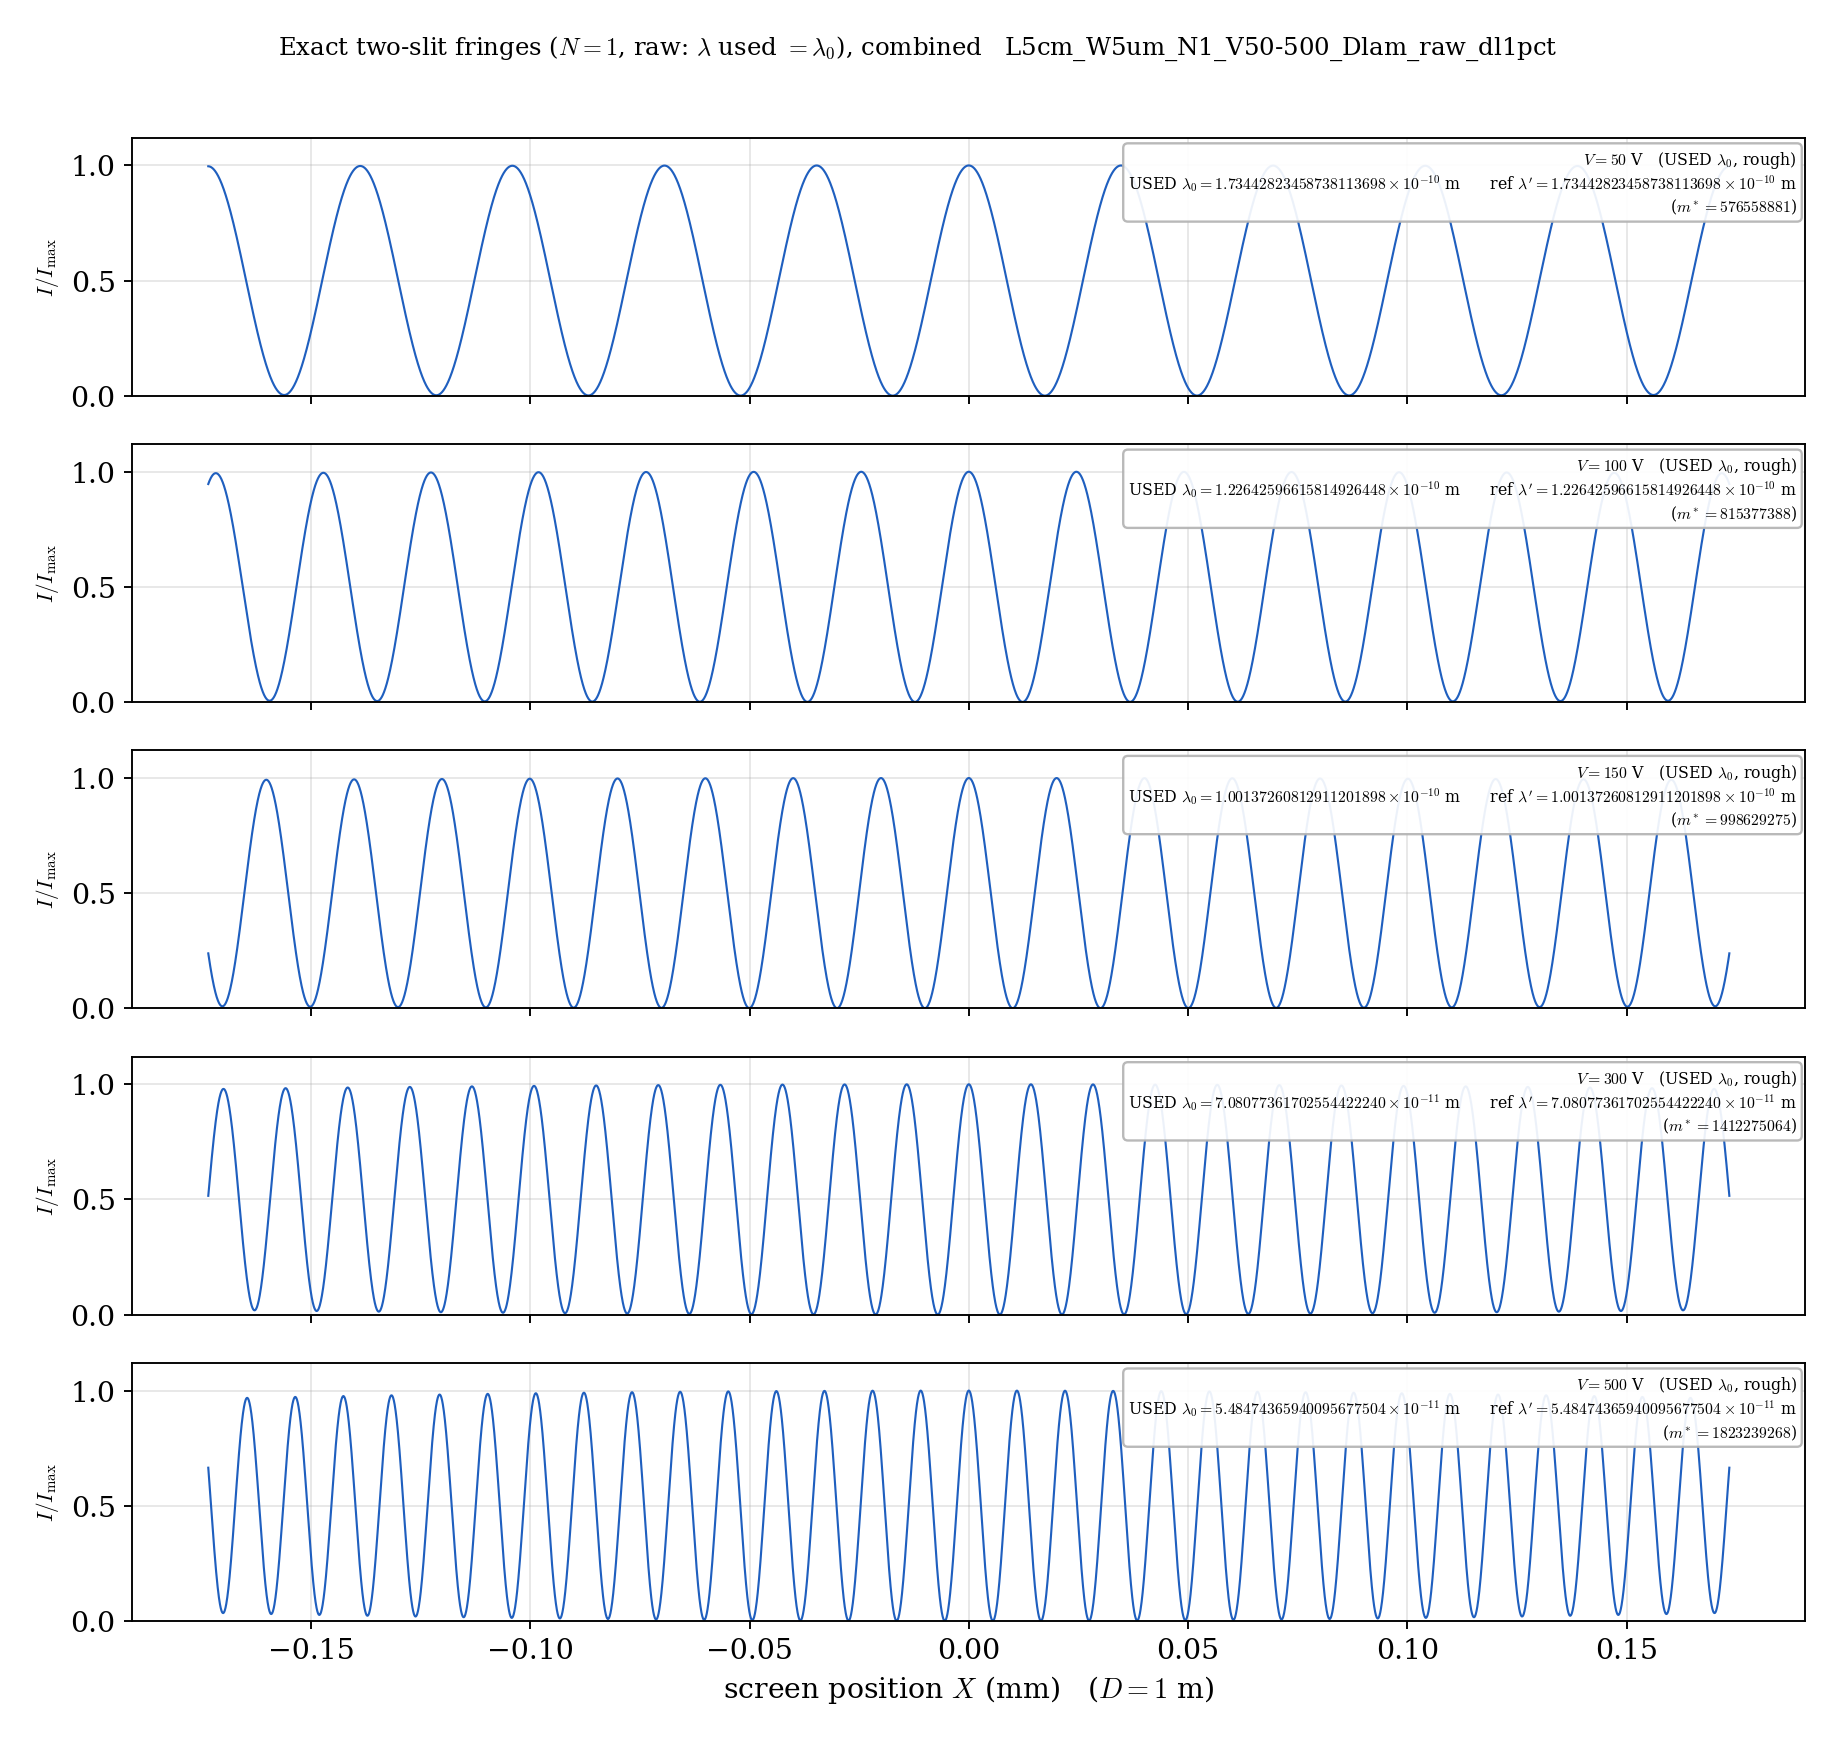
\includegraphics[keepaspectratio,alt={Figure 2}]{debroglie_fringes_combined_L5cm_W5um_N1_V50-500_Dlam_raw_dl1pct.png}}
\textbf{Figure 2}: \(N=1\) accumulated fringes
(\(V=50,100,150,300,500\,\mathrm{V}\), \(D=1\,\mathrm{m}\), common
window). Each row is the exact re-computed accumulation of 200 electrons
with source position fluctuating over \(\pm\lambda_0/2\) and wavelength
over \(\pm1\%\). Higher voltages give denser fringes
(\(\Delta X=0.035\to0.011\,\mathrm{mm}\)), and the \(\pm1\%\) wavelength
spread slightly lowers the visibility toward the window edges (§3).

\begin{center}\rule{0.5\linewidth}{0.5pt}\end{center}

\section{\texorpdfstring{4. \(N>1\): survival of interference, and
fundamental-wavelength invariance of the observed
wavelength}{4. N\textgreater1: survival of interference, and fundamental-wavelength invariance of the observed wavelength}}\label{n1-survival-of-interference-and-fundamental-wavelength-invariance-of-the-observed-wavelength}

We compute the multi-harmonic cases \(N=9,17\) (Table 1).

\textbf{Uncorrected (raw, using \(\lambda_0'\) directly)}: the
inter-harmonic absolute alignment phase
(\(r_{\mathrm{avg}}/\lambda\sim5\times10^8\)) is generally not aligned,
the localization collapses, and multiple split peaks appear. Because of
the multiple peaks \textbf{a unique period is not defined and the
wavelength cannot be read from the fringe spacing}. The
\(\mathrm{slope}/h\) obtained by formally applying the same readout is
\(0.139\) for \(N=9\) and \(0.081\) for \(N=17\), but \textbf{these are
diagnostics for a collapsed pattern with no stable fringes and do not
represent a valid wavelength measurement}.

\pandocbounded{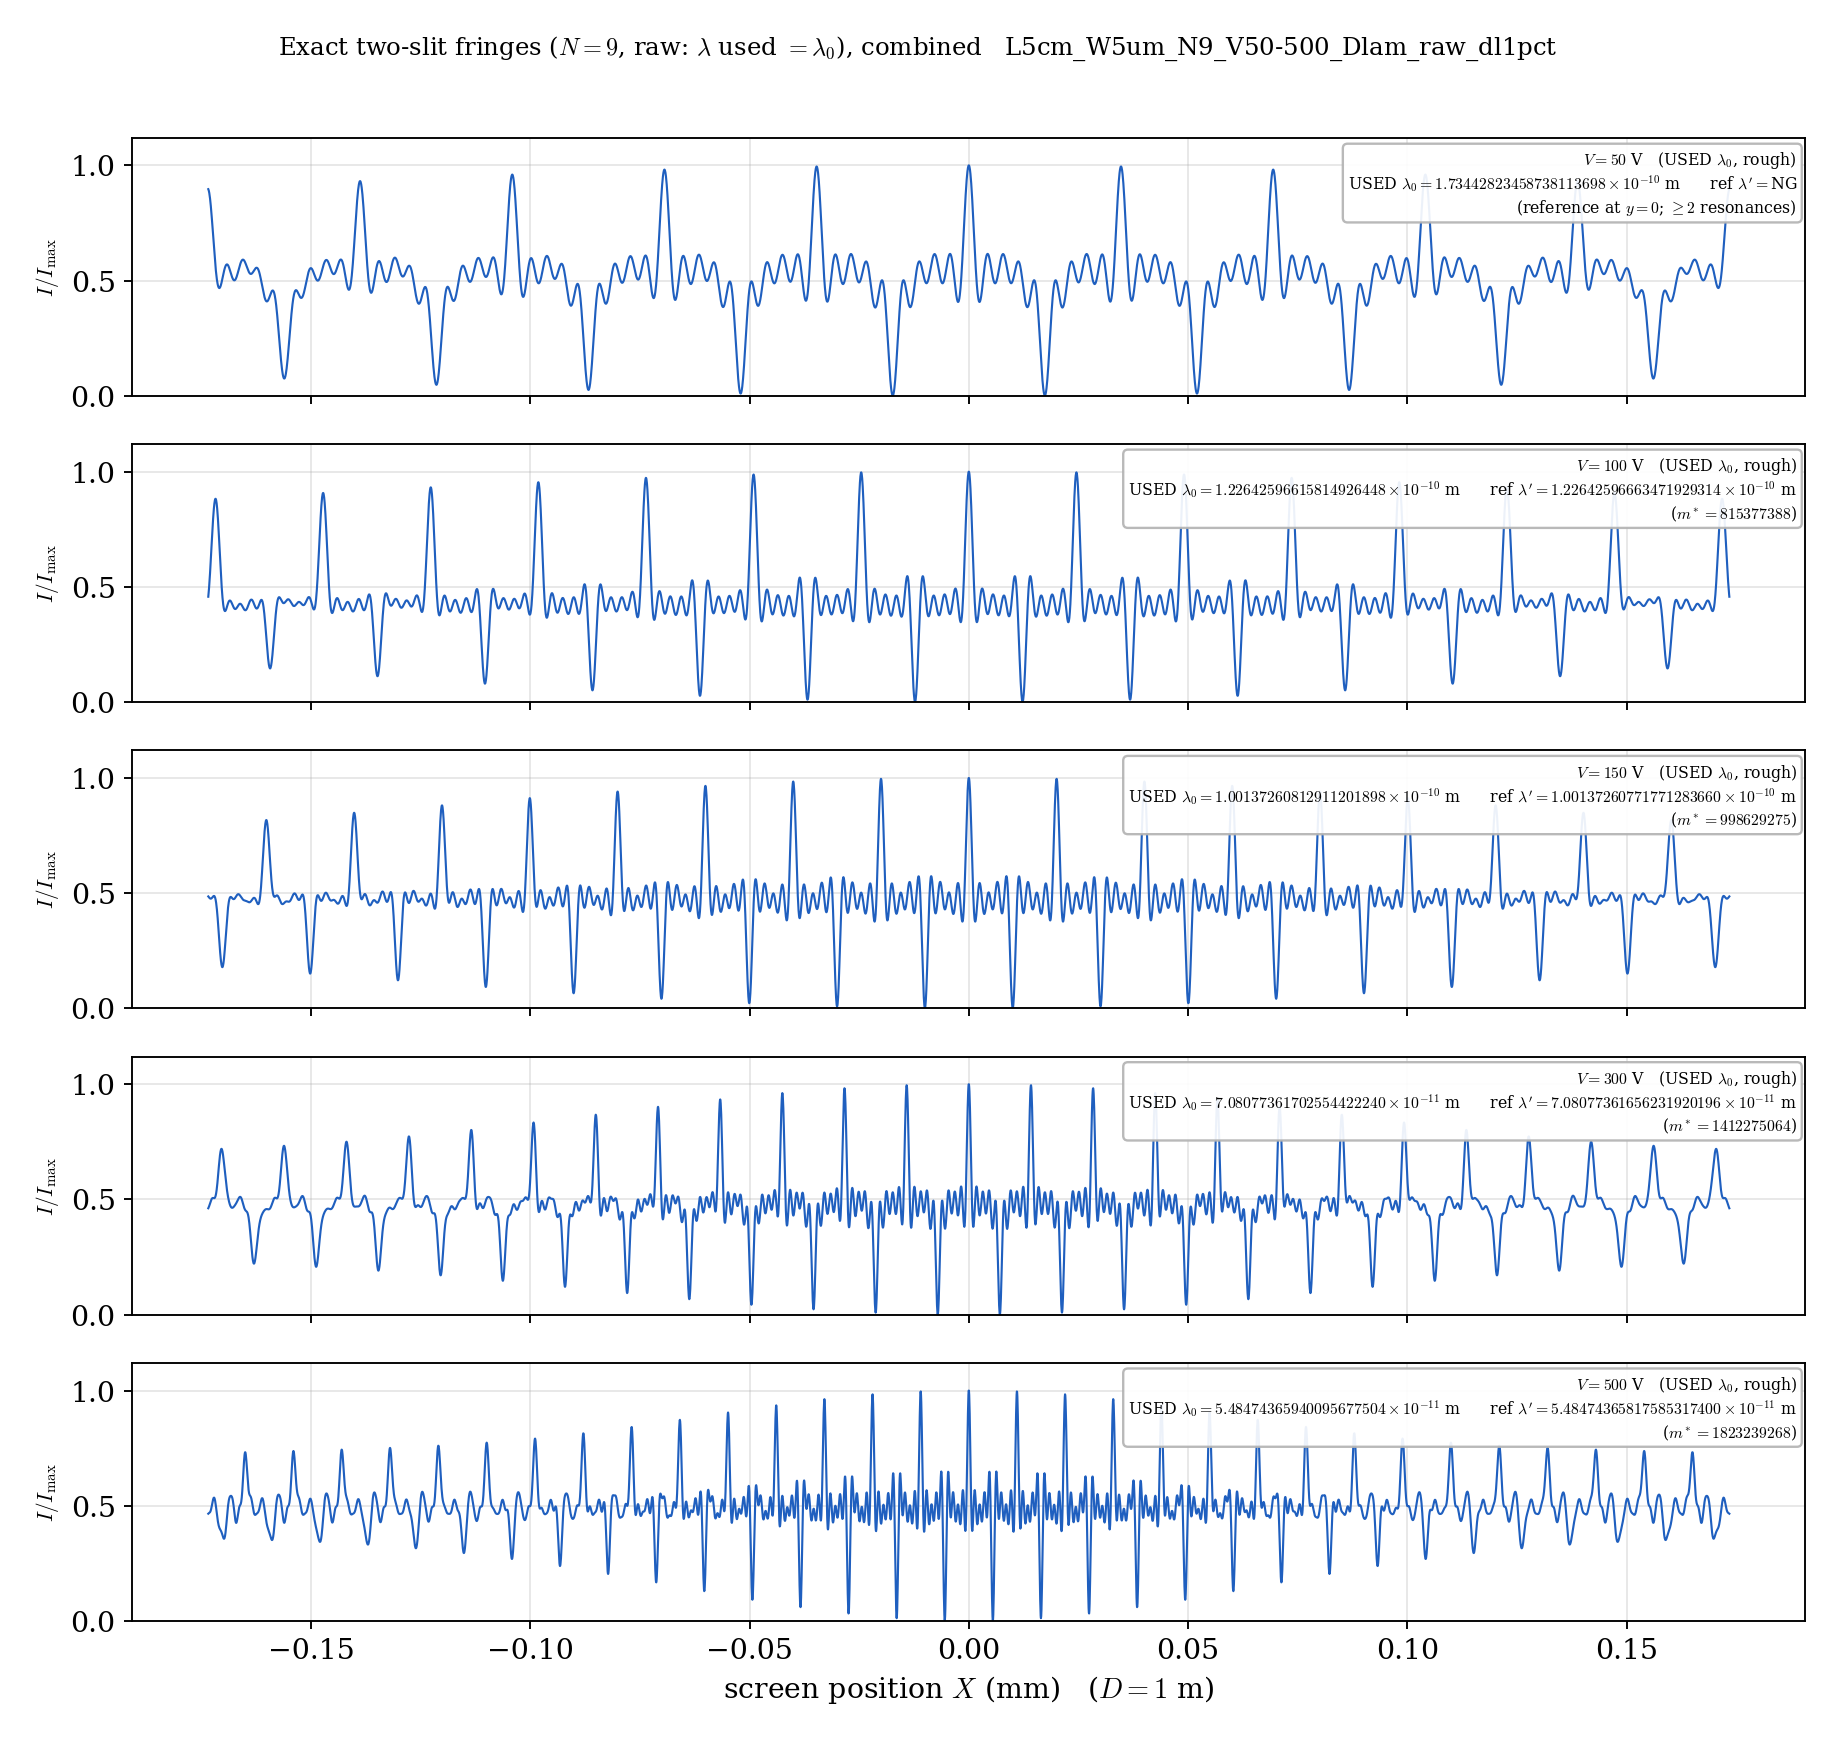
\includegraphics[keepaspectratio,alt={Figure 3}]{debroglie_fringes_combined_L5cm_W5um_N9_V50-500_Dlam_raw_dl1pct.png}}
\textbf{Figure 3}: \(N=9\) \textbf{uncorrected} (raw) accumulated
fringes. Each period is not a single sharp peak but \textbf{split
multiple peaks (comb-like)}, and the center \(s=0\) is not a main peak =
stable interference does not hold. In this state a unique period cannot
be read.

\textbf{Corrected (align, using \(\lambda'\))}: each electron's
\(\lambda_0'\) is aligned to the nearest resonance
\(\lambda'=2r_{\mathrm{avg}}/M\) of its geometry \(r_{\mathrm{avg}}(y)\)
(= the survival filter, §2.5). All harmonic phases align and a train of
sharp single localized peaks is restored (Figure 4). Reading the
wavelength geometrically from the main-peak spacing \(\Delta X\) of this
sharp train, via \(\lambda=\Delta X\cdot W/D\), agrees with the
\(\lambda'\) obtained through \(A\) (the wavelength that could not be
read in raw is recovered in align). The slope of
\(\langle p\lambda'\rangle\) is \(0.99973\) for \(N=9\) and \(0.99972\)
for \(N=17\).

\pandocbounded{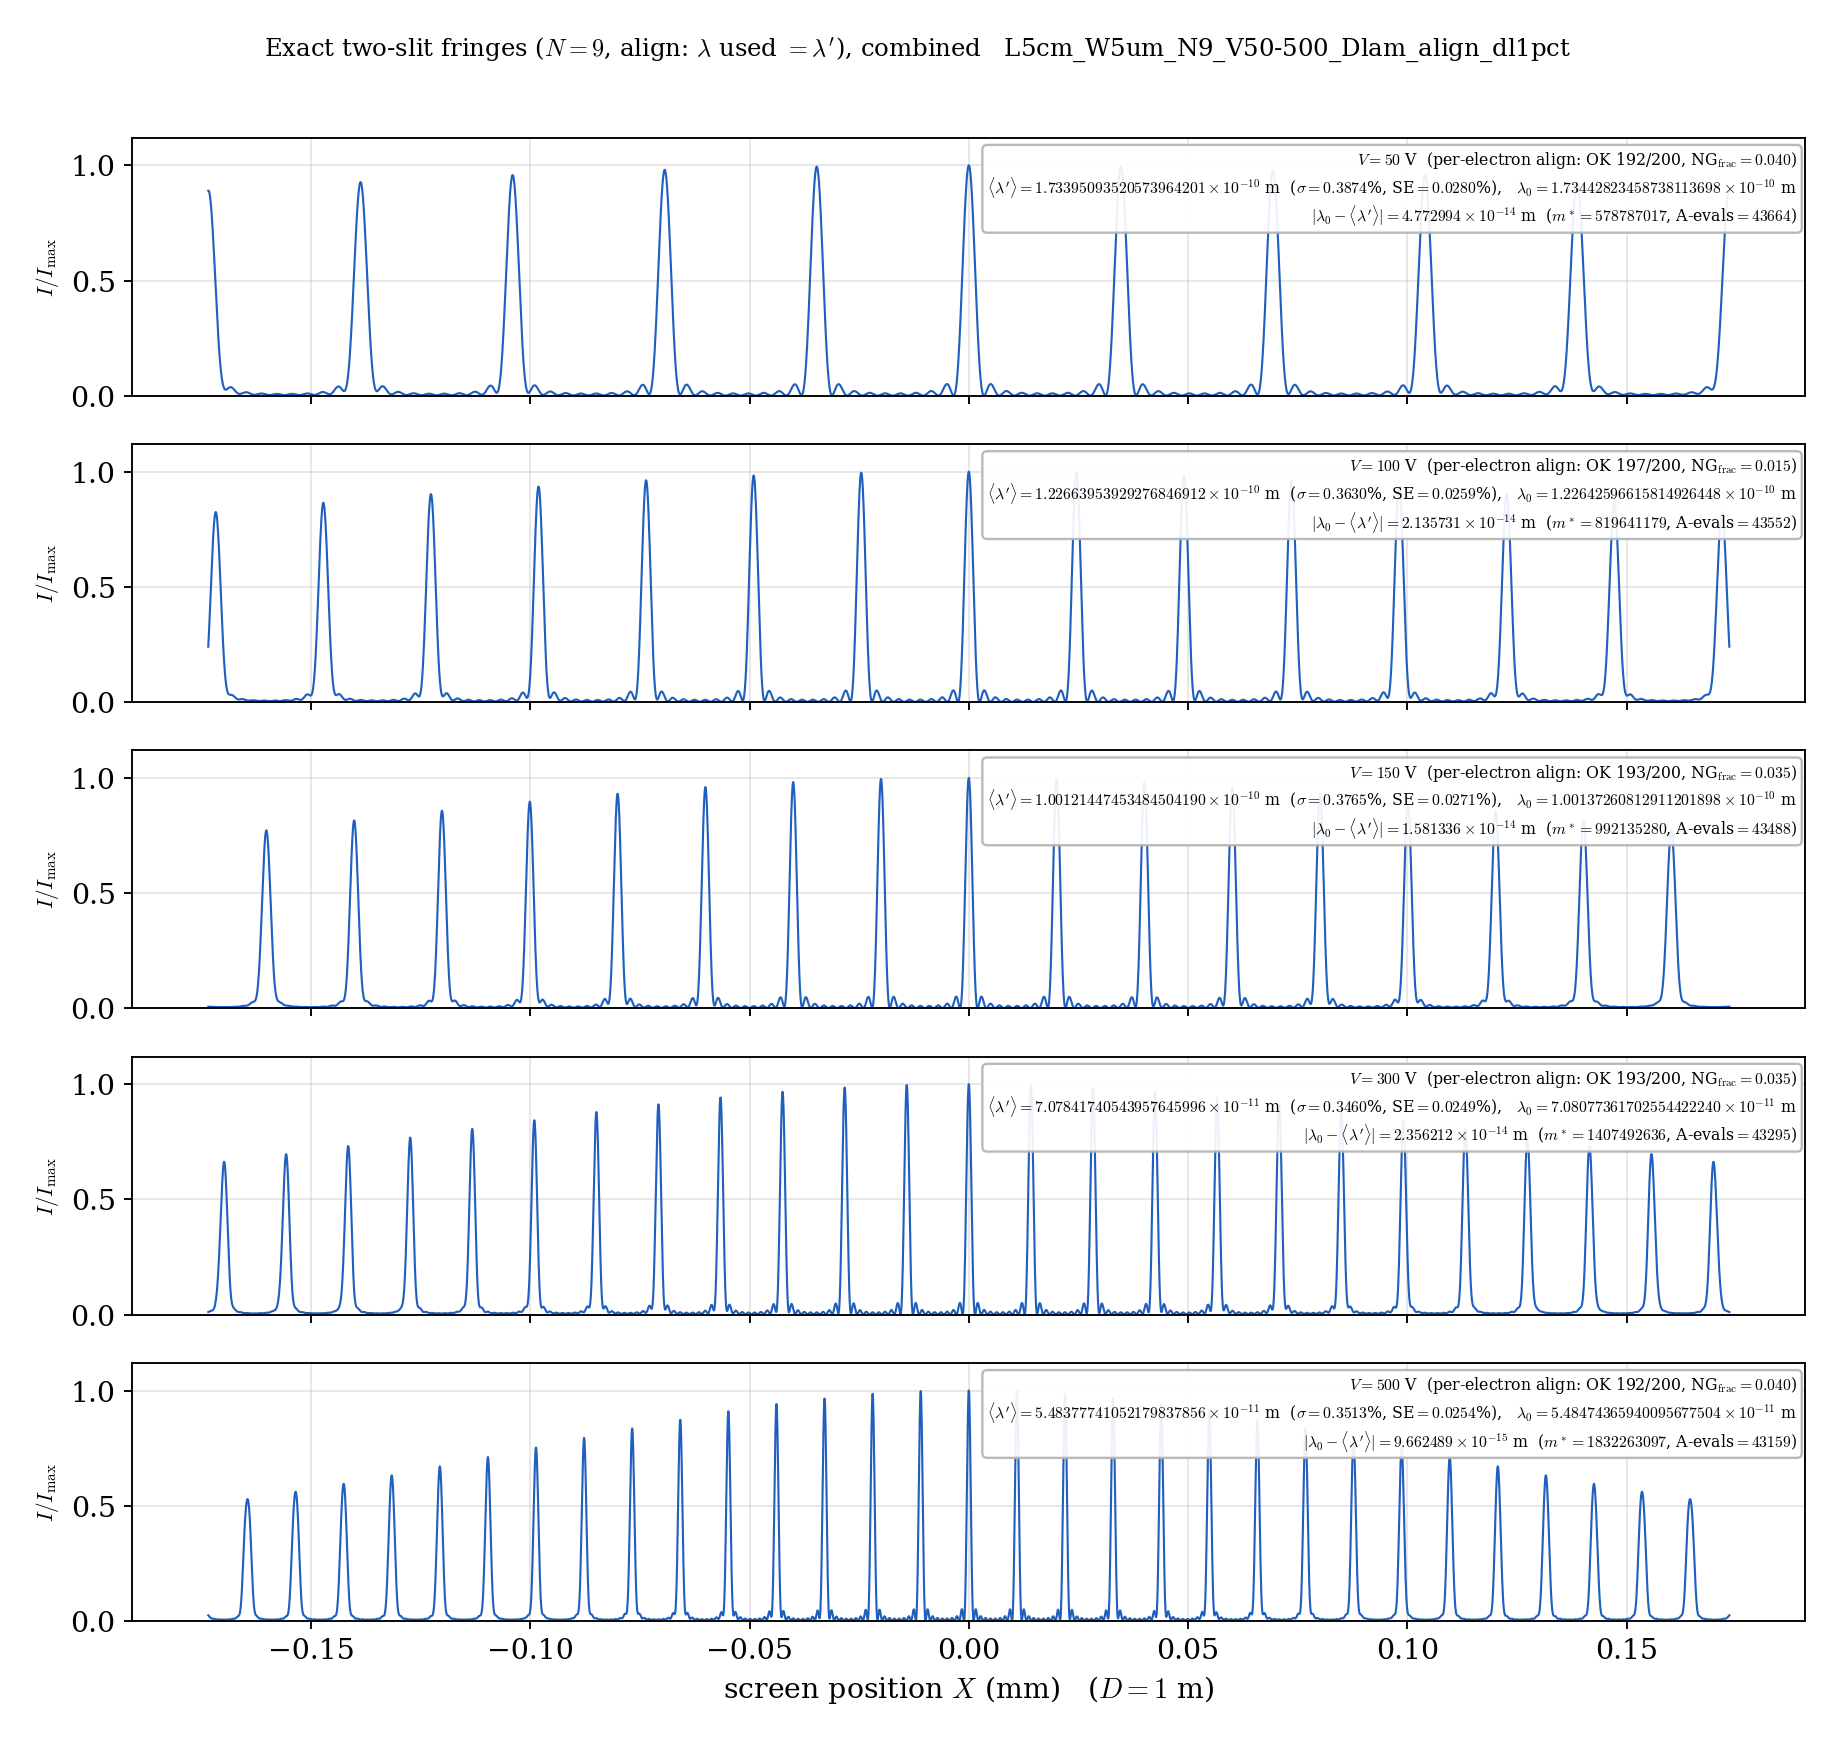
\includegraphics[keepaspectratio,alt={Figure 4}]{debroglie_fringes_combined_L5cm_W5um_N9_V50-500_Dlam_align_dl1pct.png}}
\textbf{Figure 4}: \(N=9\) \textbf{aligned} (align) accumulated fringes.
The comb-like split of Figure 3 turns, via the survival filter, into
\textbf{sharp single localized peaks (with the \(S_N\) side-lobes)}.
Each panel annotates \(n_{\mathrm{OK}}/200\), the exclusion rate,
\(\langle\lambda'\rangle\) (20 digits), \(\sigma\%\), SE\(\%\).
\(\lambda'\) coincides with \(\lambda_0\) to relative \(\sim10^{-9}\);
the alignment is a tiny snap to a geometric resonance.

\pandocbounded{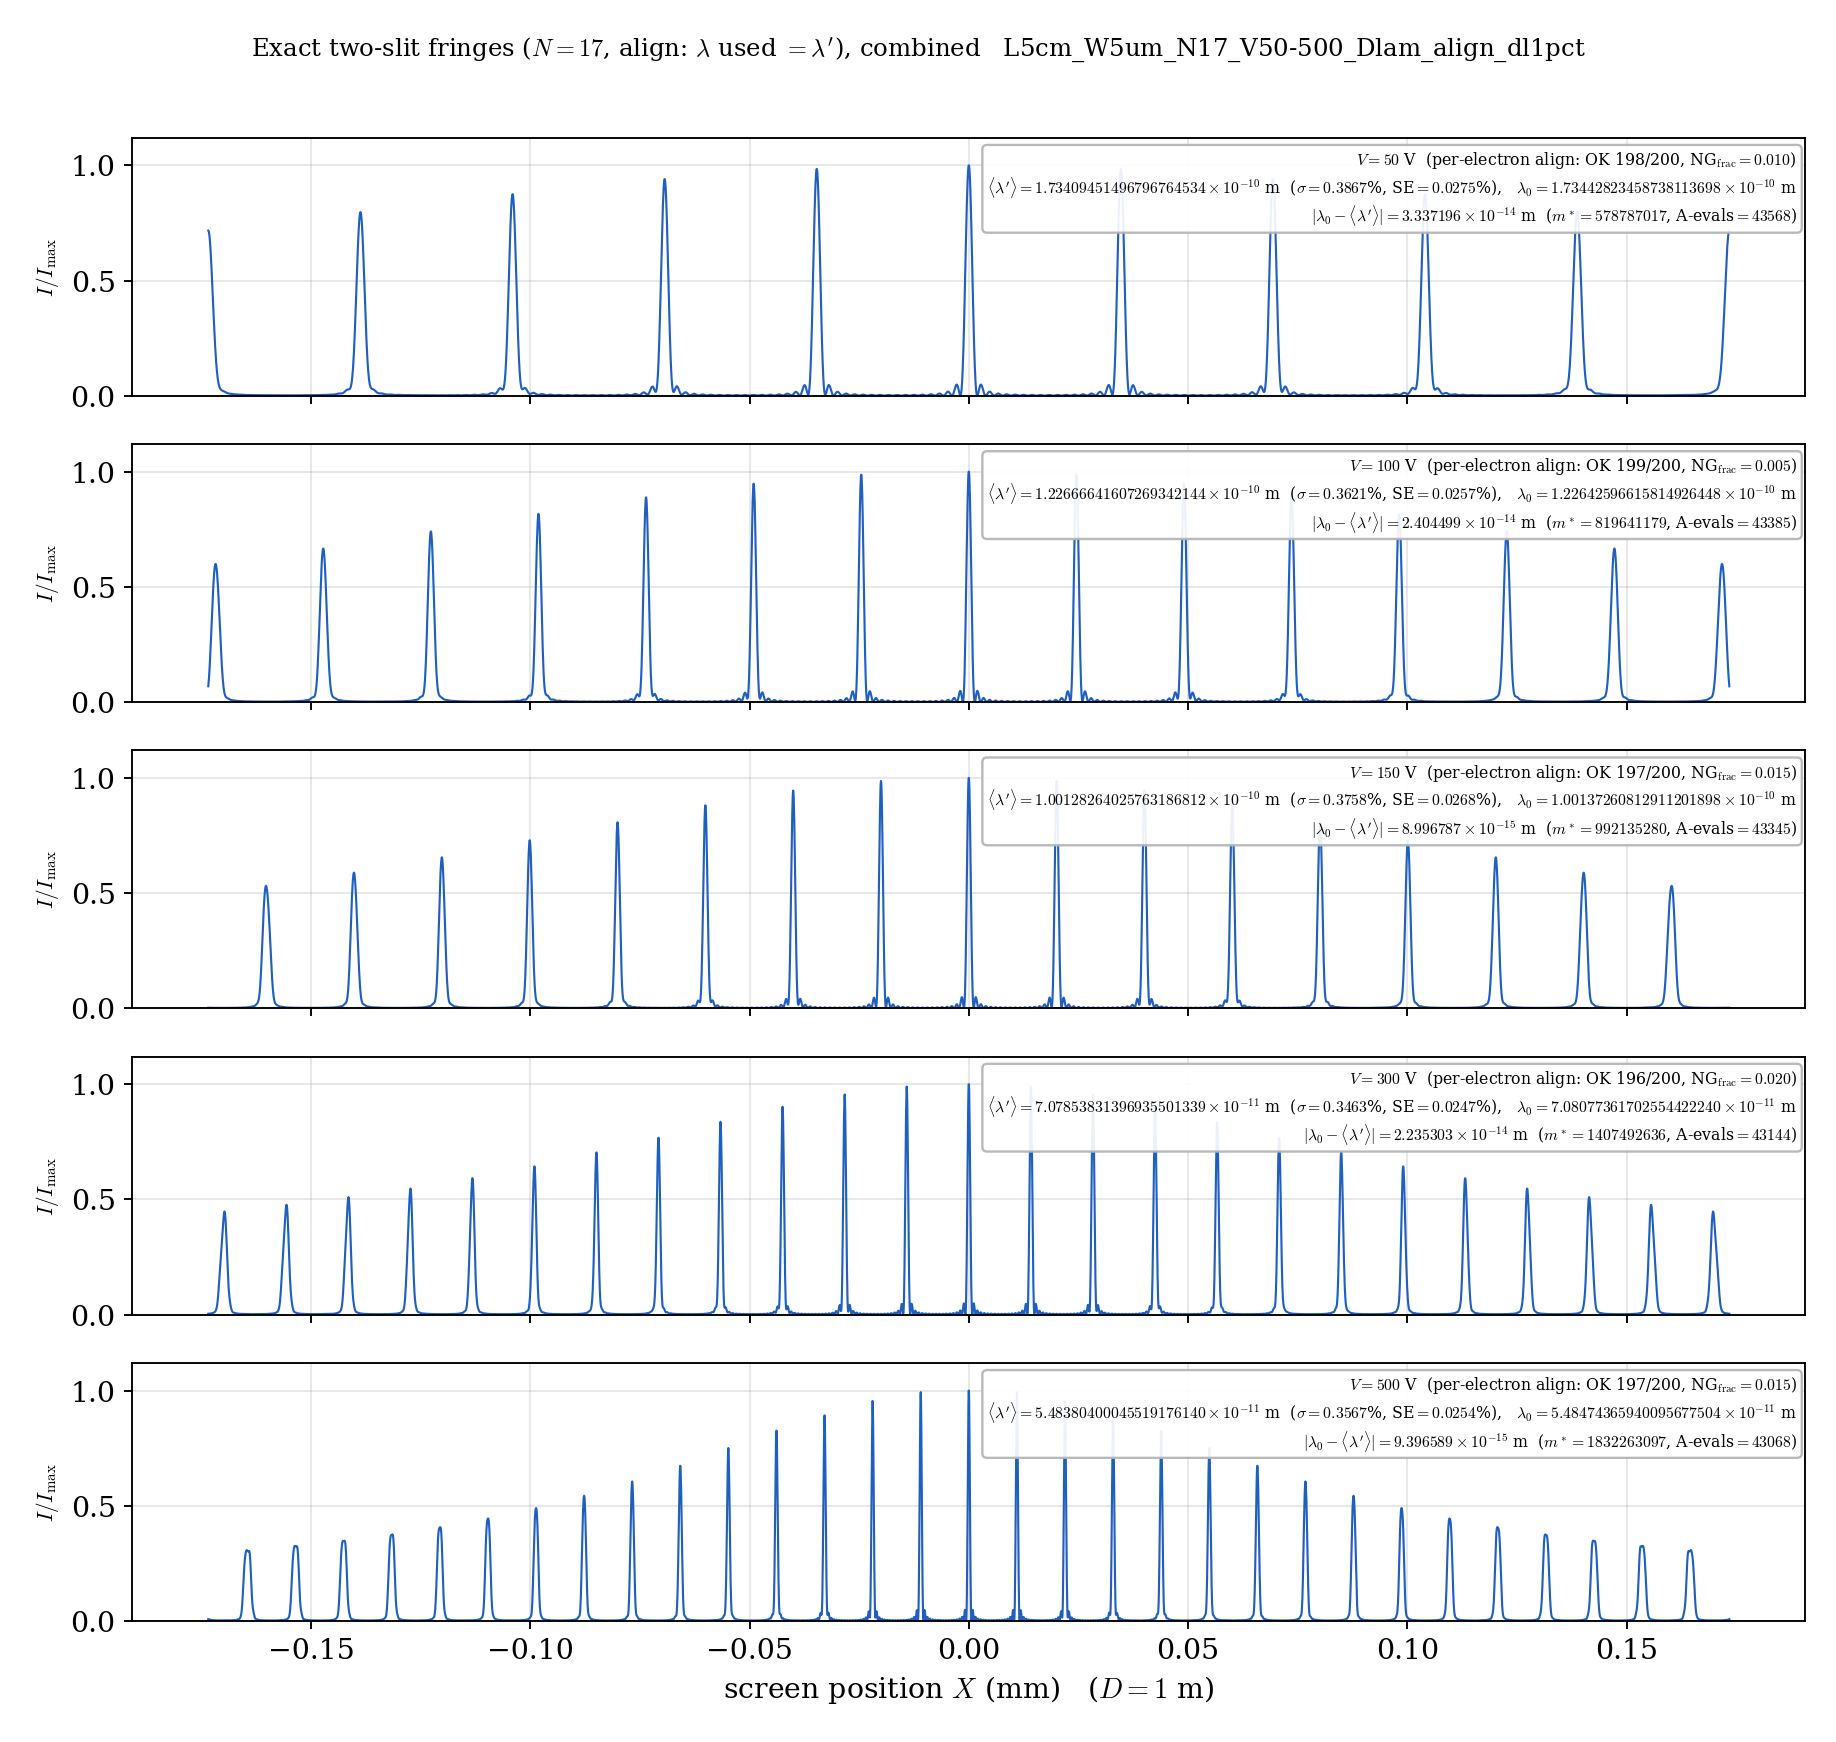
\includegraphics[keepaspectratio,alt={Figure 5}]{debroglie_fringes_combined_L5cm_W5um_N17_V50-500_Dlam_align_dl1pct.png}}
\textbf{Figure 5}: \(N=17\) aligned. With 9 harmonics the localization
is even sharper. \textbf{The peak positions and spacing are invariant
with respect to \(N\)}; \(N\) controls only the resolution (sharpness
\(\sim1/(N{+}1)\)).

{\def\LTcaptype{none} % do not increment counter
\begin{longtable}[]{@{}
  >{\raggedleft\arraybackslash}p{(\linewidth - 8\tabcolsep) * \real{0.2000}}
  >{\raggedleft\arraybackslash}p{(\linewidth - 8\tabcolsep) * \real{0.2000}}
  >{\raggedleft\arraybackslash}p{(\linewidth - 8\tabcolsep) * \real{0.2000}}
  >{\raggedleft\arraybackslash}p{(\linewidth - 8\tabcolsep) * \real{0.2000}}
  >{\raggedleft\arraybackslash}p{(\linewidth - 8\tabcolsep) * \real{0.2000}}@{}}
\toprule\noalign{}
\begin{minipage}[b]{\linewidth}\raggedleft
\(N\)
\end{minipage} & \begin{minipage}[b]{\linewidth}\raggedleft
\# harmonics \(K\)
\end{minipage} & \begin{minipage}[b]{\linewidth}\raggedleft
raw \(\mathrm{slope}/h\) (diagnostic)
\end{minipage} & \begin{minipage}[b]{\linewidth}\raggedleft
align \(\mathrm{slope}/h\)
\end{minipage} & \begin{minipage}[b]{\linewidth}\raggedleft
localization width \(\sim1/(N{+}1)\)
\end{minipage} \\
\midrule\noalign{}
\endhead
\bottomrule\noalign{}
\endlastfoot
1 & 1 & \(0.99977\) & \(0.99977\) & sinusoid (no localization) \\
9 & 5 & \(0.139\) (collapsed, invalid) & \(0.99973\) & \(\sim1/10\) \\
17 & 9 & \(0.081\) (collapsed, invalid) & \(0.99972\) & \(\sim1/18\) \\
\end{longtable}
}

\textbf{Table 1}: \(N\) dependence of \(\mathrm{slope}/h\) (\(\pm1\%\)
wavelength fluctuation, 200-electron average). \textbf{The raw values
are formal readouts of a collapsed pattern and are not wavelength
measurements.} When aligned, \(\mathrm{slope}/h\approx1\) regardless of
\(N\).

After alignment, the main-peak positions on the screen are given by
\(Ws/\lambda'\in\mathbb{Z}\), so the main-peak spacing in the paraxial
coordinate \(X\simeq Ds\) is \(\Delta X=\lambda' D/W\). The odd-harmonic
count \(N\) changes the sharpness and the side-lobe structure, but this
\textbf{main-peak spacing is set by the fundamental wavelength
\(\lambda'\) alone and is independent of \(N\)}.

\textbf{Central result of this section (a structural result independent
of the origin of \(\lambda_0\))}: increasing \(N\), the spacing of the
sharp localized-peak train after align (= the central fringe spacing
\(\Delta X=\lambda_0 D/W\)) is set by the fundamental wavelength
\(\lambda_0\) and is independent of the harmonic count \(N\). That is,
even when finer internal structure (harmonics) than \(\lambda_0\) is
packed in, the wavelength scale observed under two-slit geometry is
\textbf{invariant} as the fundamental wavelength, and what \(N\) changes
is only the sharpness of localization (resolution). The trade-off
\textbf{high \(N\) = high resolution but high fragility (tolerance band
\(\sim1/(2N)\))} could be compared in future work with the
resolution--stability trade-off of atomic clocks and electron
interferometers (this paper makes no detailed comparison) {[}1{]}.

\begin{center}\rule{0.5\linewidth}{0.5pt}\end{center}

\section{\texorpdfstring{5. \(p\) vs \(1/\lambda\) and the simulated
observation of \(p\lambda\)
constancy}{5. p vs 1/\textbackslash lambda and the simulated observation of p\textbackslash lambda constancy}}\label{p-vs-1lambda-and-the-simulated-observation-of-plambda-constancy}

\pandocbounded{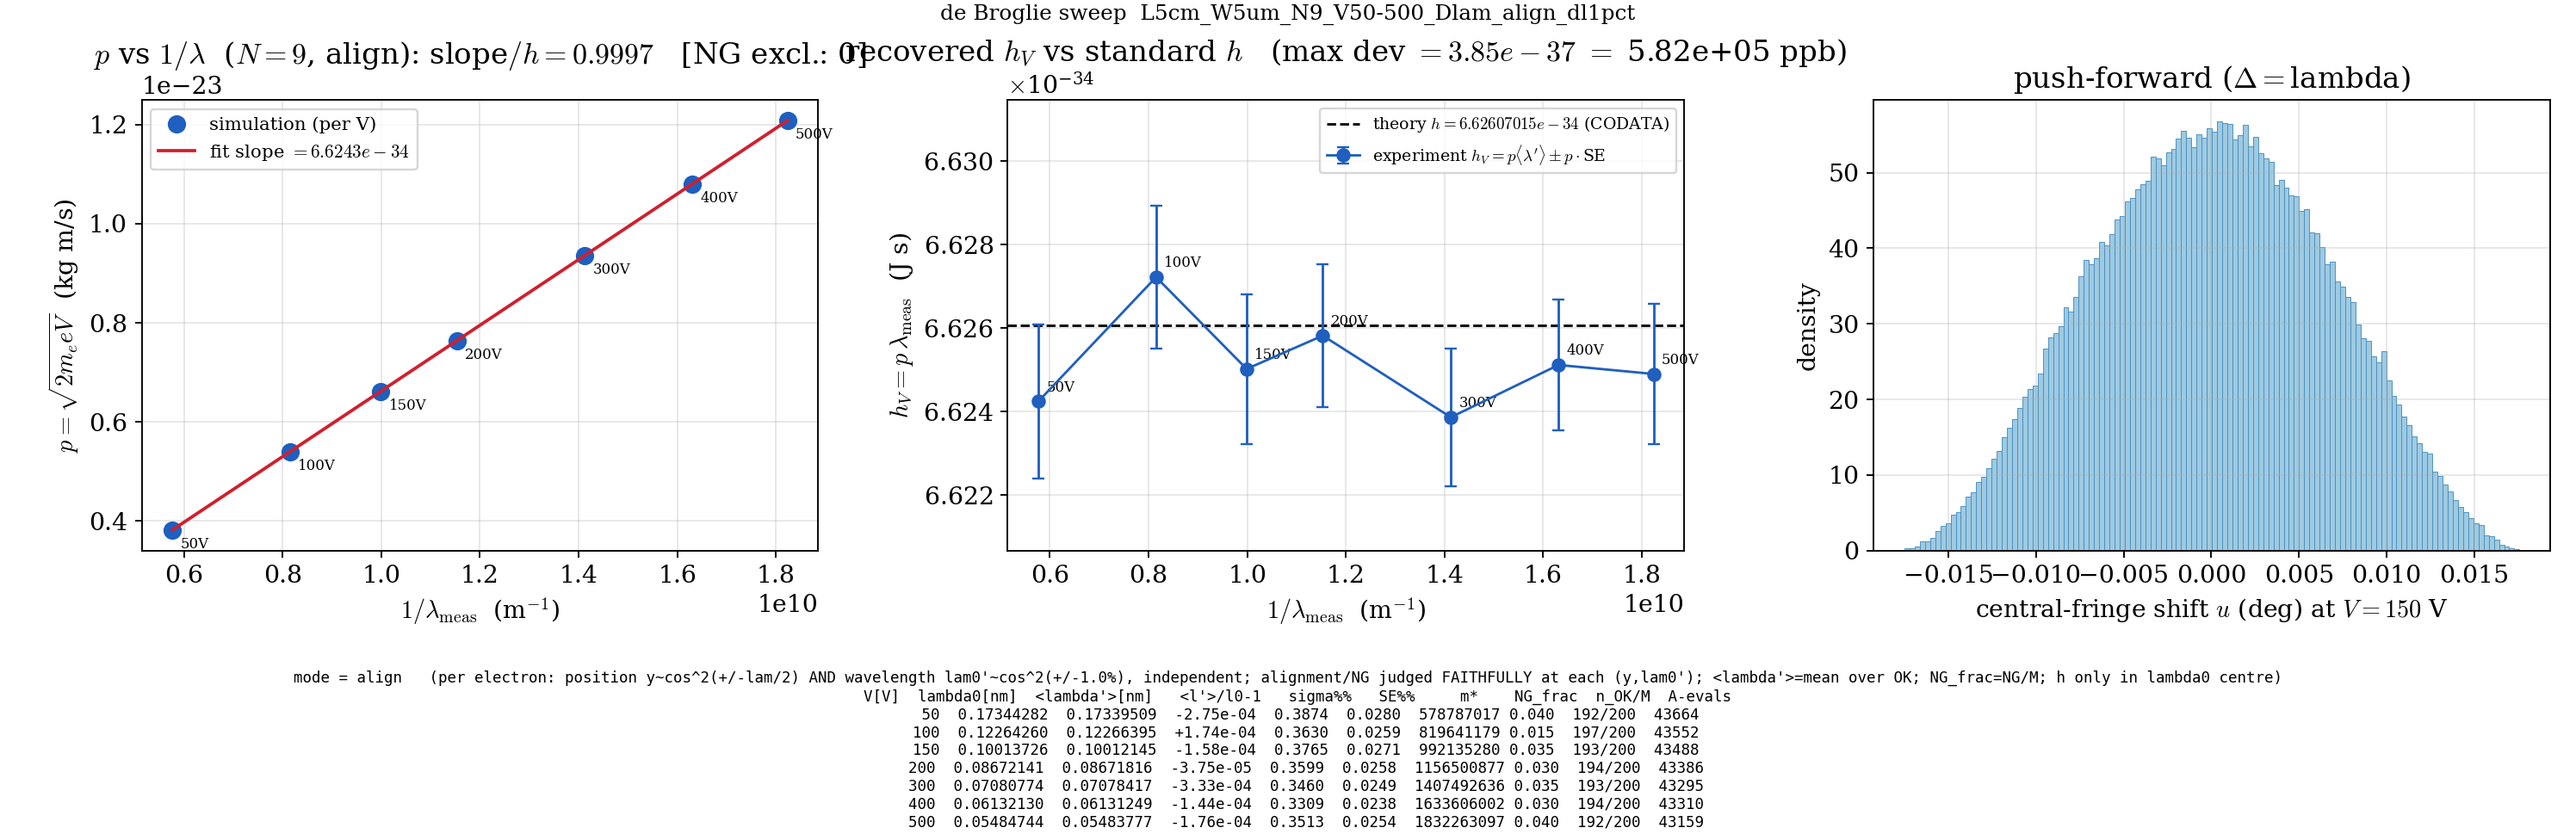
\includegraphics[keepaspectratio,alt={Figure 6}]{debroglie_sweep_L5cm_W5um_N9_V50-500_Dlam_align_dl1pct.png}}
\textbf{Figure 6}: Summary of \(N=9\) align (\(\pm1\%\) wavelength
fluctuation, 200 electrons per voltage). \textbf{How to read (three
panels)}: \textbf{Left} = \(p\) vs \(1/\langle\lambda'\rangle\) (a
straight line, slope \(=h\)). The linearity is a visualization of the
relation, not a measure of precision. \textbf{Center} = the per-voltage
\(h_V=p\langle\lambda'\rangle\) plotted with \(\pm p\cdot\)SE error
bars, extremely zoomed around CODATA \(h\) (dashed, at the center). All
error bars contain \(h\), so \(\langle p\lambda'\rangle\) is
statistically consistent with \(h\) (scatter \(\sim0.03\%\) = the
200-average of the \(\pm1\%\) input). \textbf{Right} = the distribution
of the central-fringe positional shift caused by the source-position
fluctuation (\(\cos^2\)). The bottom table gives, per voltage,
\(\langle\lambda'\rangle\), \(\sigma\%\), SE\(\%\), exclusion rate,
\(n_{\mathrm{OK}}/200\), and the number of \(A\) evaluations.
Representative values: \(\sigma\approx0.35\text{–}0.39\%\) (matching the
theoretical \(0.362\%\)), SE \(\approx0.025\text{–}0.028\%\), exclusion
rate \(1.5\text{–}4.0\%\), \(n_{\mathrm{OK}}=192\text{–}197/200\).

\subsection{5.1 Explicit statement of
self-consistency}\label{explicit-statement-of-self-consistency}

We use \(\lambda_0=h/p\) as the \textbf{center} of each electron's
initial wavelength \(\lambda_0'\). \(h\) enters at this single place and
returns as \(p\lambda'\approx h\) through \(\lambda'\approx\lambda_0\)
(snap \(\sim10^{-9}\)). Hence ``recovering \(h\)'' is itself
\textbf{self-consistent (circular)} and is not an independent numerical
determination of \(h\). The \(\pm1\%\) wavelength fluctuation and the
200-electron average are a realism device against misreading; the
many-electron average \(\langle p\lambda'\rangle\to h\) is a consequence
of the cancellation due to \(\lambda_0'\) being symmetric about the
center \(\lambda_0=h/p\) (interference does not independently select or
correct the true value \(h\)). The \textbf{survival of the structure and
the fundamental-wavelength invariance} discussed in §4 are separate
results that do not depend on this circularity.

\subsection{5.2 What this paper does not derive (scope of the
claim)}\label{what-this-paper-does-not-derive-scope-of-the-claim}

\textbf{(a) Not a first-principles derivation of \(p\lambda=h\).}
\(p=\sqrt{2m_eeV}\) is the classical momentum set by the accelerating
voltage (no \(h\)), and \(\lambda\) is the representative wavelength
\(\lambda_0=h/p\) given to the source and the effective wavelength
\(\lambda'\) extracted from interference. Since \(\lambda_0\) itself is
given using \(h\), \(p\lambda'\approx h\) is a self-consistent result
and is not a derivation that \(h\) emerges from the conjugacy of \(p\)
and \(\lambda\).

\textbf{(b) Not a derivation of a \(\Delta x\,\Delta p\sim h\) type
uncertainty relation.} What the localized odd-harmonic wave of this
paper essentially possesses is only the \textbf{classical (Fourier)
relation \(\Delta x\,\Delta k\sim1\)} between the localization width
\(\Delta x\) and the wavenumber width \(\Delta k\). To connect this to a
momentum width and obtain \(\Delta x\,\Delta p\sim\hbar\) requires, as a
separate physical input, \(p=\hbar k\) (= the de Broglie correspondence
itself). This paper is a stage that assumes it, and does not derive the
uncertainty relation.

Therefore what this paper shows is a classical-wave-model result:
\textbf{even when finer localized odd-harmonic structure than
\(\lambda_0\) is given to a wave whose representative wavelength is at
the de Broglie scale, it survives stably as sharp interference under
two-slit geometry and alignment, and the simulated-observed central
fringe spacing is invariant as the fundamental wavelength
\(\lambda_0\)}---it is neither a derivation of the value \(h\) nor a
derivation of conjugacy / uncertainty.

\subsection{5.3 Correspondence with real experiments (a limited
analogy)}\label{correspondence-with-real-experiments-a-limited-analogy}

Davisson--Germer and other real matter-wave experiments also narrow the
wavelength range by coarse estimation and then increase precision by
lattice diffraction, but in real experiments the diffraction angle, an
external measured datum, supplies \(\lambda\) independently. This model
generates fringes from \(\lambda_0=h/p\) and reads them back, so it has
no independent measurement path and is not isomorphic in this respect.
The exclusion (NG) and per-electron alignment are not a model of quantum
measurement or wave-packet collapse but a classical filtering operation
of ``adopting only trials in which stable interference held'', and can
be positioned as one concrete example of the quantum--classical
correspondence (§2.5, §7).

\begin{center}\rule{0.5\linewidth}{0.5pt}\end{center}

\section{6. Limits of the computation and the
model}\label{limits-of-the-computation-and-the-model}

\begin{itemize}
\tightlist
\item
  \textbf{Self-reference}: since the center of \(\lambda_0'\) is
  \(h/p\), the numerical value of \(h\) is not determined independently.
\item
  \textbf{Triviality from lattice density}: since the resonance-lattice
  spacing \(\sim10^{-19}\,\mathrm{m}\) is dense,
  \(\lambda'\approx\lambda_0\) is mathematically almost inevitable. The
  claim of this paper is placed not on ``recovering a value'' but on
  ``interference survival of the localized structure and
  fundamental-wavelength invariance'' (§4, §7). Computing in a
  coarse-lattice regime (drastically smaller \(L\), or an analogous
  experiment at optical wavelengths) would make the deviation between
  \(\lambda'\) and \(\lambda_0\) visible and highlight the
  non-triviality of the mechanism (future work).
\item
  \textbf{Numerical precision}: since
  \(r_{\mathrm{avg}}/\lambda\sim10^9\), the alignment phase for \(N>1\)
  is at the float64 limit; \(A(\lambda)=I(0)/4K^2\) (absolute alignment)
  is computed and \(\lambda'=2r_{\mathrm{avg}}/M\) is constructed
  directly to avoid cancellation.
\item
  \textbf{Non-countability of the order \(M\)}: \(M\sim10^9\) is unlike
  the small orders \(n=1,2,3\) of Bragg diffraction and cannot be
  identified by counting fringes, so it is not fully isomorphic to
  crystal Bragg diffraction.
\item
  \textbf{Smallness of the push-forward}: the fringe shift for the
  source-position fluctuation \(\pm\lambda_0/2\) (a basic assumption of
  this paper) is \(\sim0.02^\circ\), small because of paraxiality, and
  its contribution to the central wavelength scale is small (a correct
  consequence under the assumption).
\item
  \textbf{Representative values}: \(L,W,V,\Delta,\delta\) are
  representative values, so the quantitative precision is limited.
\end{itemize}

\begin{center}\rule{0.5\linewidth}{0.5pt}\end{center}

\section{7. Conclusion and outlook}\label{conclusion-and-outlook}

In a single-source double-slit classical wave model, we gave a localized
odd-harmonic wave (\(N>1\)) with a de Broglie-scale representative
wavelength \(\lambda_0=h/p\), and fluctuated each electron's position
(\(\pm\lambda_0/2\)) and wavelength (\(\pm1\%\)) independently to
compute the interference, alignment, and exclusion exactly. \(N=1\) is a
check of the procedure. \textbf{The central result of this paper is not
the value of \(h\), but (i) that a classical wave with structure finer
than \(\lambda_0\) can survive stably as a sharp single-peak
interference under two-slit geometry, and (ii) that the central spacing
of the surviving fringes remains at the fundamental wavelength
\(\lambda_0\), invariant with respect to the harmonic count \(N\) (\(N\)
controls only the resolution \(\sim1/(N{+}1)\)).} Under a symmetric
fluctuation centered at \(\lambda_0=h/p\), \(\langle p\lambda'\rangle\)
agrees with \(h\) within the standard error, but this is a
self-consistency due to lattice density and not an independent
derivation.

\textbf{This paper is neither a first-principles derivation of
\(p\lambda=h\) nor a derivation of a \(\Delta x\,\Delta p\sim h\) type
uncertainty relation.} The value of this paper is not that it ``derived
\(h\)'', but that it \textbf{verified, in an explicit classical wave
model, that even with localized structure finer than the de Broglie
wavelength, the observed interference wavelength remains at the de
Broglie scale (fundamental-wavelength invariance).}

Outlook: (a) visualize \(\lambda'\ne\lambda_0\) in a coarse-lattice
regime (small \(L\) / optical wavelengths) to show the non-triviality of
the mechanism, (b) quantify the \(N\)- and
fluctuation-width-\(\delta\)-dependence of the exclusion rate, (c)
position the alignment sensitivity (high resolution and high fragility)
as a universal structure shared with atomic clocks and electron
interferometers, (d) publish an English version.

\begin{center}\rule{0.5\linewidth}{0.5pt}\end{center}

\section{References}\label{references}

{[}1{]} N. Kihara, \emph{Localized odd-harmonic wave and the alignment
condition in a single-source double-slit model}, Zenodo (2026). DOI:
\href{https://doi.org/10.5281/zenodo.21035831}{10.5281/zenodo.21035831}.
(The exact title, DOI, and publication status should be finalized
against the deposit.)

{[}2{]} C. Davisson and L. H. Germer, ``Diffraction of Electrons by a
Crystal of Nickel,'' \emph{Physical Review} \textbf{30}, 705--740
(1927). DOI: 10.1103/PhysRev.30.705.

{[}3{]} L. de Broglie, ``Recherches sur la théorie des quanta,''
\emph{Annales de Physique} \textbf{10}(3), 22--128 (1925). DOI:
10.1051/anphys/192510030022. (The formal journal information / DOI
should be verified.)

{[}4{]} M. Born, ``Zur Quantenmechanik der Stoßvorgänge,''
\emph{Zeitschrift für Physik} \textbf{37}, 863--867 (1926). DOI:
10.1007/BF01397477. --- In this paper the \(\cos^2\) probability density
used for the source-position distribution is referenced as an assumption
of a \textbf{Born-type (\(|\psi|^2\)-type) probability distribution}
(§2.4). It does not derive or apply the Born rule itself.

\begin{center}\rule{0.5\linewidth}{0.5pt}\end{center}

\emph{Note: the numerics and figures were generated by the parameterized
\texttt{debroglie\_plambda\_sweep.py} (exact two-slit intensity +
independent \(\cos^2\) fluctuation of position and wavelength +
per-electron accumulation) and the absolute-alignment \(A\) search
solver \texttt{debroglie\_align\_lambda.py}. The generation condition of
each figure is encoded in its filename
(e.g.~\texttt{...\_N9\_V50-500\_Dlam\_align\_dl1pct} = \(N{=}9\),
aligned, wavelength fluctuation \(\pm1\%\)).}
\end{document}
